Because this is a project about Hamiltonian Monte Carlo, imagine a frictionless puck on an icy surface of varying heights. The state of this puck is given by it's momentum $\bm{q}$ and position $\bm{p}$. The potential energy of the puck $U$ will be a function of only its height, while the kinetic energy will be a function of its momentum $K(q)=\frac{|\bm{q}|^2}{2m}$. If the ice is flat, the puck will move with a constant velocity. If the ice slopes upwards, the kinetic energy will decrease as the potential energy increases until it reaches zero, at which point it will slide back down. In the context of Bayesian statistics, we can think of the position of the puck as the posterior distribution we want to sample from, and the momentum variable are artificial constructs that allow us to efficiently move around our space. We use the notion of position and momentum, jointly called the Hamiltonian system, to propose samples where we set $U(p) = -\log[P(p)\mathcal{L}(p|\mathcal{D})]$\\

The final algorithm will be:

\begin{algorithm}[H]
	\KwIn{Starting position $\theta^{(1)}$ and step size $\epsilon$.}
	\For{t=1, 2, \dots} {
		Sample momentum $r^{(1)}\sim\mathcal{N}(0, M)$\\
		$r_0=r_0+\frac{\epsilon}{2}\Delta U(\theta_0)$\\
		\For{i=1,\dots,m} {
			$\theta_i=\theta_{i-1}+\epsilon M^{-1}r_{i-1}$\\
			$r_i = r_{i-1} - \epsilon  \Delta U(\theta_i)$\\
		}
		$r_m = r_m -\frac{\epsilon}{2}\Delta U(\theta_m)$\\
		$(\hat{\theta}, \hat{r})=(\theta_m,r_m)$\\
		Sample $u\sim\mathrm{Uniform}[0, 1]$\\
		$\rho = \exp\braces{H(\hat{\theta}, \hat{r})-H(\theta^{(t)}, r^{(t)})}$\\
		\If{$u < \min(1, \rho)$}{$\theta^{(t+1)} = \hat{\theta}$}
	}
\end{algorithm}




\begin{figure}[H]
\centering
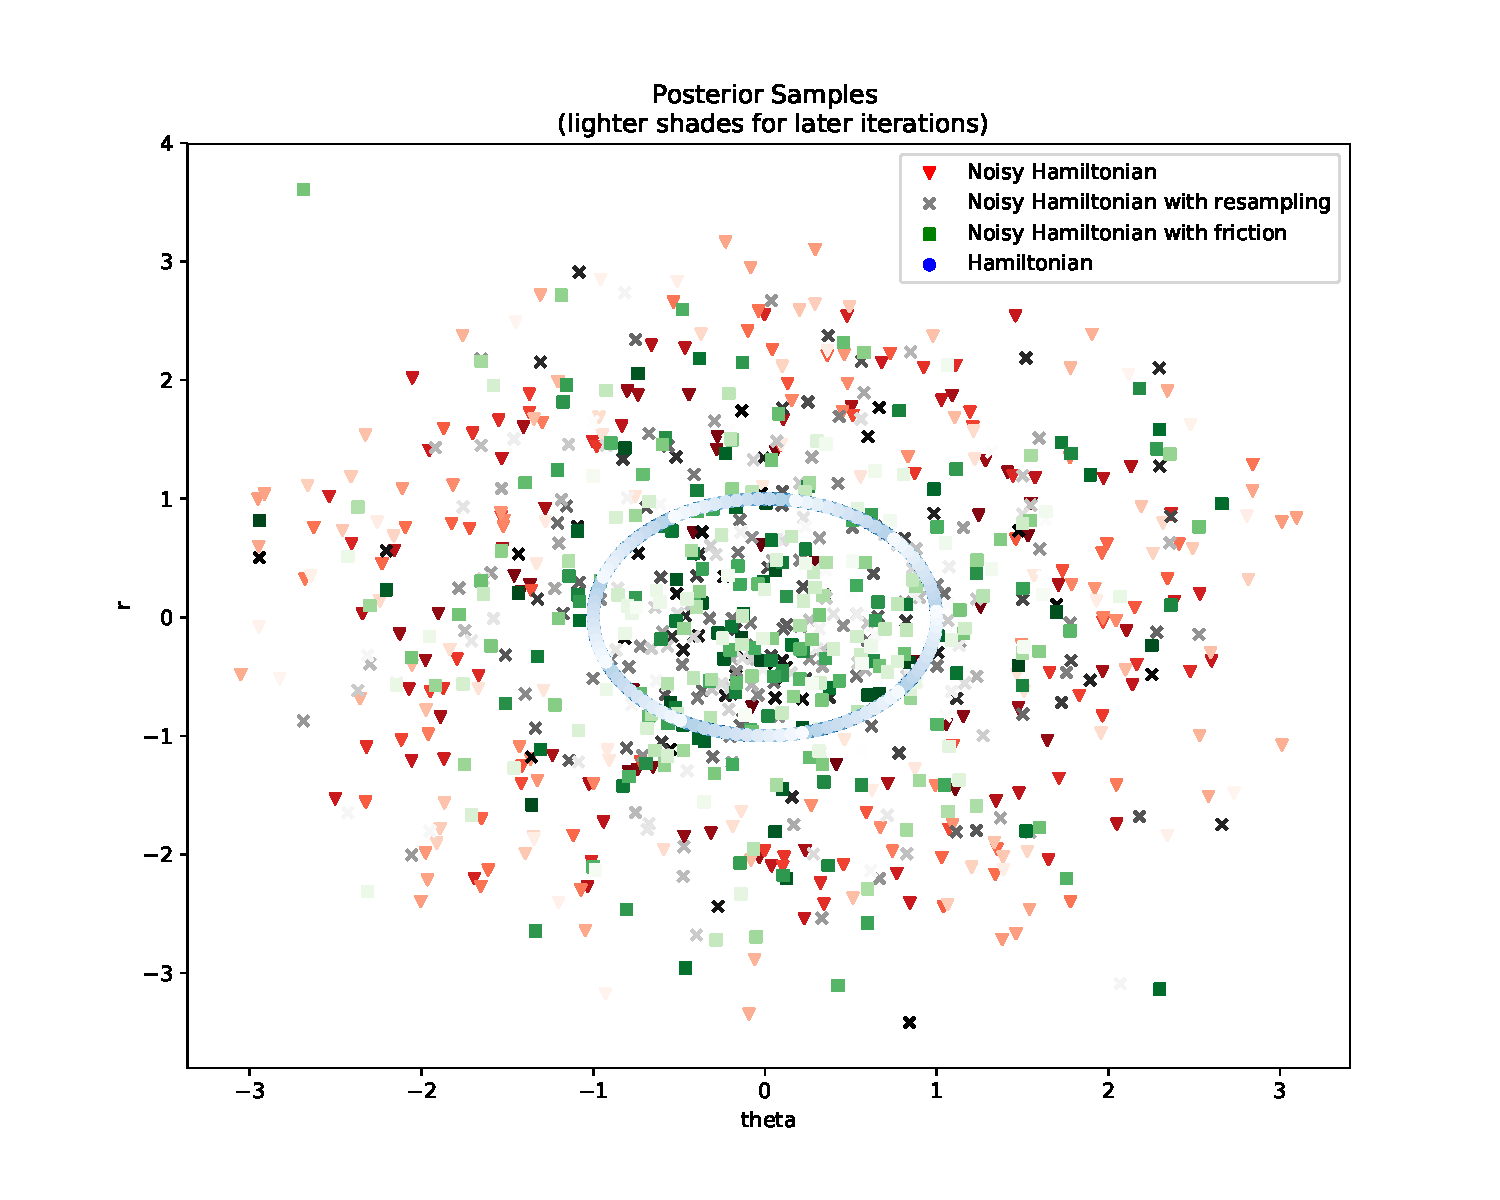
\includegraphics[width=0.9\textwidth]{posterior_samples.pdf}
\end{figure}
